\chapter{Future Works}	
  \section{Studies of 2011 PbPb data}

    \subsection{High mass $\gamma-\gamma \rightarrow e^{+} e^{-}$  in PbPb 2011}
      A study of the di-electron production in UPC events is already possible 
	from the recorded 2011 data. 
      This measurement would make use of the electron triggers and combined the 
	current di-muon data with di-electron data from the triggers using the
	ECAL. 
      The electron triggered sample potentially offers a large increase in 
	statistics. 
      By adding the additional channel the statistics would already increase.
      However in addition to this, because of the smaller mass of the electron,
	di-electron production is slightly favor compared to di-muon 
	production.
      STARlight predicts that di-electron cross section is a factor of more than 
	2.5 higher in Xn break-up mode than the di-muons channel when looking 
	at masses above 4 GeV.
      The acceptance for electrons in potential higher as well. 
      The ECAL is position just beyond the tracker, whereas the muon system is 
	outermost sub-detector. 
      This elevates the main reduction of muon acceptance, which is the material
	budget. 
      There is simply a lot a detector in front the muon system.

      In order to perform the study several key additions would need to be made
	relative to the current di-muon analysis. 
      The original reconstruction of the data used in the current di-muon 
	analysis does not contain electron objects. 
      Either the analysis would have to migrated to reconstruction of the data
	done in a newer software version, or reconstruction of the electrons 
	would have to be added to the current analysis chain. 
      There are currently no electron UPC MC samples produced. 
      In order to study the acceptance and efficiency for electrons these samples
	would be need. 
      The ultimate limitation on this study is the 2 GeV threshold in $p_{T}$ in
	the ECAL trigger. 
      This limits the di-electron mass range to where the trigger is efficient. 

      The contribution of higher order diagrams can be explored by the 
	photoproduction of di-lepton pairs is to explore.
      With additional contributions to the physics communities understanding of 
	this process this study will help to determine necessity or 
	non-necessity of including higher order of corrections in simulations 
	such as STARlight.
      Having an additional channel to help constrain the current di-muon measure 
	of the of UPC $\gamma-\gamma$ interaction will also help to constrain 
	the $J/\psi$ measurement by adding a data driven check on the 
	normalization $\gamma-\gamma$ background to the $J/\psi$
      
    \subsection{UPC Hadronic Overlap and PbPb 2011}
      In the model calculations explored in this analysis of UPC quarkonia 
        photoproduction all hadronic interactions are rejected.
      Photoproduction in events where hadronic interactions occur are not 
        included in the cross section calculation.
      However, inclusive $p_{T}$ spectra of $J/\psi$ measured by ALICE in 
        peripheral PbPb collisions show a low momentum peak consistent with 
				coherent photoproduction ~\cite{aliceIclJpsi}.
			\begin{figure}[h]
				\centering
				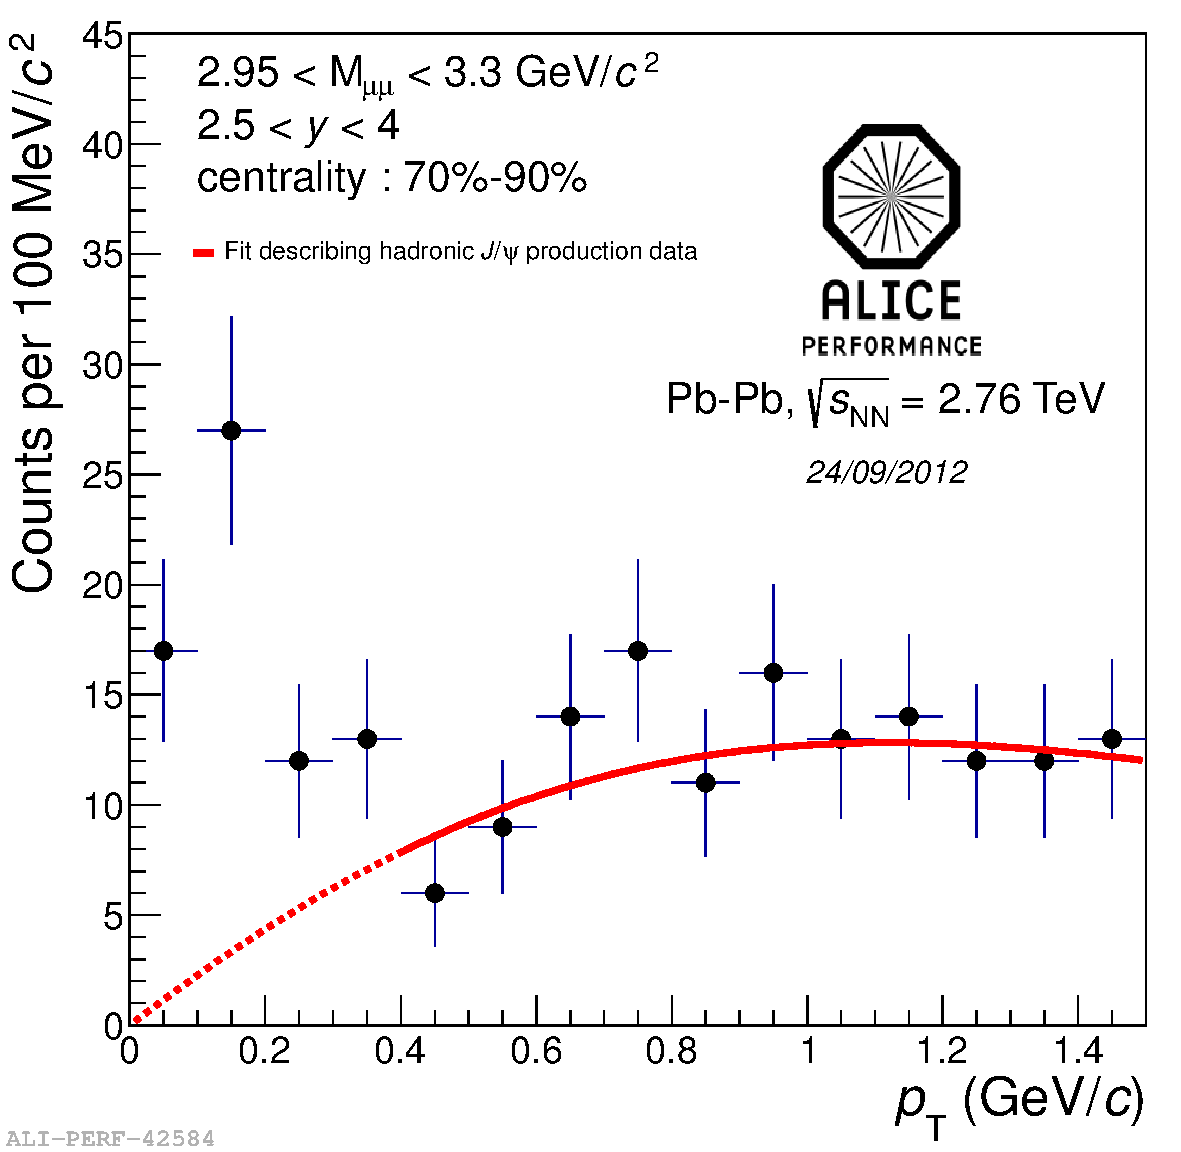
\includegraphics[width=0.5\textwidth]{2012-Sep-24-excess7090.pdf}
				\caption{Coherent excess in inclusive $J/\psi$ $p_{T}$ spectrum.}
				\label{fig:alicePtSpecLowPt}
			\end{figure}
		  CMS has the opportunity to explore this overlap between hadronic 
				interactions and photoproduction using PbPb data from 2011 that is 
				already recorded.

      To study the overlap between photoproduction and hadronic proctuction of 
				quarkonia event the inelastic sample and the UPC sample could both be
				used. 
      The looseness of the veto designed to reject hadronic interactions,
        which uses the BSC detector, leaves a significant overlap with 
				peripheral hadronic collisions. 
      The inclusive quarkonia sample from typical hadronic collisions can also 
        be utilized. 
      Coherent quarkonia photoproduction has a distinctive low $p_{T}$ structure
				that can be used to identify photoproduced candidates in a sample that 
				contains photoproduction combined with hadronic interactions.
      This measurement would open up the door to exploring the boundary between
				photoproduction and hadronic production.
      By looking at the mixing of the two, both process, hadronic production and 
				photoproduction, will be better understood.

      In order to compliment each others strengths, the inclusive hadronic sample 
				and the UPC sample of dimuon candidates would be utilized in this study.
      The two samples muon and centrality biases are orthogonal allowing each to 
				serve as a check on the other. 
      The inclusive hadronic sample is triggered by a higher $p_{T}$ threshold 
				double trigger, whereas the UPC sample is uses a lower $p_{T}$ single 
				muon trigger.
      The UPC sample is strongly biased toward peripheral events, which would 
				lead to inefficiencies as events become more central, whereas, the 
				inclusive sample is slightly biases in the most peripheral events due to
				an inefficiency an event selection efficiency in the most peripheral 
				centrality bin.
      If these offsetting biases can be exploited, clarity about the transition 
				between and mixing of photoproduction and hadronic production of 
				quarkonia can be produced. 
      A measurement of the kind proposed here will both produce a better 
				understanding of the low $p_{T}$ portion of the inclusive spectrum as 
				well as the hadronic overlap with UPC measurements.

    \subsection{UPC with muons in HF}
      As higher rapidities are explored both lower and higher momentum partons
        of the nucleus are probed. 
      Because these two contributions to the UPC photoproduction cross-section 
        can be separated using neutron tagging in incoherent events, exploring
				higher dimuon rapidities becomes attractive.
      HF extends to 5 in $\eta$, 2.6 units beyond the edge of the tracker.
      By combining hits in HF with tracks in the tracker the higher dimuon 
        rapidities could be explored. 
      When combined with neutron tagging of incoherently produced quarkonia,
        the current study can be extended to probe lower-x nuclear partons 
			  by identifying muons in HF. 

  \section{Studies of 2013 pPb data and 2015 PbPb data}
	  Specific UPC triggers were also developed for the pPb run in 2013. 
		For this period of running a much higher total trigger rate was read out 
		  relative to 2011.
		The total rate allocated for UPC triggers at the L1 in 2013 was 5kHz and 
		  50 Hz at the HLT.
		This factor of 5 increase in the bandwidth, especial in L1 rate, allowed for
		  a different triggering strategy than in 2011. 

    The basic strategy in 2013 was the same as in 2012, use the loosest 
		  available ECAL and muon L1 triggers to push to capture the lowest $p_{T}$
			electrons and muons possible.
		Because of the L1 bandwidth restrictions in 2011, both the ZDC and the BCS 
		  were used on the L1 to reduce rates.
		In 2013 only the muon and ECAL triggers were used on the L1 allowing for 
		  rejection of hadronic interactions through cuts on track multiplicity. 
		In addition, a more sophisticated trigger using full dimuon reconstructed 
		  was developed to increase purity.
		The main advantage in this shift in strategy is the increase in cross 
		  section that is gained by removing the ZDC requirement out of the trigger.

		The PbPb run in 2015 will be at higher beam energies and luminosities.
		The $sqrt{s_{NN}}$ will increase from 2.76 TeV in 2011 to 5.1 TeV with
		  a project integrated luminosity between $0.3/nb$ and $1/nb$. 
    The factor of 2 to 10 increase in integrated luminosity will increases the 
		  number of events directly.
		In addition, both the increase in energy, which increases the photon flux,
		  and the ability to utilize the 2013 trigger strategy of sifting the 
			onus of the trigger selection to the HLT will increase the cross section
			relative to 2012.
		The higher beam energy, higher integrated luminosity, and added selectivity
		  of the HLT will create the opportunity to explore both $J/\psi$ with 
			greater statistical precision and rarer objects such as upsilons. 

    \subsection{pPb J/Psi}
    
    \subsection{UPC J/Psi 2015}
    \subsection{UPC Upsilon 2015}
